\section{Method}
\label{sec:method}

In this section, we first provide an overview of the \thistool{} framework, and then describe in detail how the framework is implemented.
\begin{figure*}[t]
    \centering
    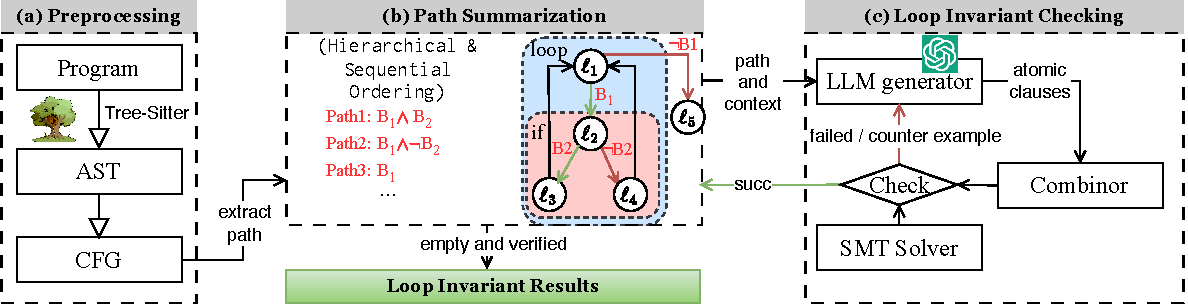
\includegraphics[width=1.00\textwidth]{figures/method_overview.pdf}
    \caption{Overview of \thistool{}.}
    \label{fig:method_overview}
%     \begin{verbatim}
% int main (){
%     int i, j, n, k, b;
%     n = 0; b = 0;
%     assume(k > 0); assume(k < 20000001);
%     assume(i == j);
%     while (n < (2 * k)){
%         n = n + 1;
%         if(b == 1){
%             b = 0; i = i + 1;
%         } else {
%             b = 1; j = j + 1;
%         }
%     }
%     if(n >= (2 * k))
%         assert(i == j);
% }
%     \end{verbatim}
\end{figure*}
\subsection{Overview}


Figure~\ref{fig:method_overview} shows the framework overview of \thistool{} comprising the following three major phases:

\textbf{(a) Preprocessing.} Our approach begins by parsing the source code into an Abstract Syntax Tree (AST) using \textsc{Tree-sitter}~\cite{max_brunsfeld_2025_17180150}, which is then transformed into a Control Flow Graph (CFG) capturing both structural and execution relationships within the program. The CFG is traversed to extract all execution paths that encode branch sequences according to the program’s hierarchical and sequential structure (see Section~\nameref{sec:PathStore}).

\textbf{(b) Path Summarization.} Each path is independently analyzed by the LLM to generate clause-level invariants. Paths corresponding to inner or earlier control structures, such as the innermost loops or the first encountered branches, are assigned higher priority to ensure that their invariants are generated and verified first. 
Verified invariants are recorded as summaries for subsequent paths, allowing the LLM to leverage contextual knowledge during reasoning. Because each path corresponds to only a small program fragment, this path-based summarization improves reasoning accuracy and scalability.

\textbf{(c) Loop Invariant Checking.} After all paths are processed, the collected invariants and the complete source code are provided to the LLM to infer refined, program-level invariants. These candidates are combined and verified through an SMT solver. If verification fails, counterexamples are fed back to the LLM to guide correction—either by strengthening weak invariants or revising incorrect ones. This iterative \textit{generate–verify–refine} process continues until valid invariants are obtained or the computation times out.

% The reason we still use the LLM at the final stage, rather than directly combining the path-level invariants, is twofold. First, if the loop invariants generated at the path level are not sufficiently strong, the LLM can refine them using information from the source code. Second, since path conditions may interact or change across different paths, the LLM can leverage a holistic view of the entire program to produce more accurate and consistent final invariants.





\begin{algorithm}[t]
\caption{FindAllPaths in a Control Flow Graph (CFG)}
\label{alg:findallpaths}
\begin{algorithmic}[1]
\REQUIRE Control Flow Graph $CFG$ with entry node $CFG.entry$
\ENSURE List of all execution paths $Paths$
\STATE $Paths \gets \varnothing$
\STATE $node \gets CFG.entry$
\WHILE{$node \neq$ null}
    \IF{$node.out\_degree > 1$}
        \IF{$node$ is a loop header}
            \STATE $loopCFG \gets$ \textsc{ExtractLoopCFG}($node$)
            \STATE $loopPaths \gets$ \textsc{FindAllPaths}($loopCFG$)
            \STATE $Paths \gets Paths \cup loopPaths$
        \ELSE 
            \STATE $trueCFG \gets$ \textsc{GetTrueCFG}($node$)
            \STATE $falseCFG \gets$ \textsc{GetFalseCFG}($node$)
            \STATE $truePaths \gets$ \textsc{FindAllPaths}($trueCFG$)
            \STATE $falsePaths \gets$ \textsc{FindAllPaths}($falseCFG$)
            \STATE $branchPaths \gets truePaths \cup falsePaths$
            \STATE $Paths \gets Paths \cup branchPaths$
        \ENDIF
    \ELSIF{$node.out\_degree = 1$}
        \STATE \textsc{AddToContext}($node$)
    \ENDIF
    \STATE $node \gets node.successor$
\ENDWHILE
\RETURN $Paths$
\end{algorithmic}
\end{algorithm}



% \begin{algorithm}[t]
% \caption{FindAllPaths in a Control Flow Graph (CFG)}
% \label{alg:findallpaths}
% \KwIn{Control Flow Graph CFG with entry node CFG.entry}\\
% \KwOut{List of all execution paths Paths}\\
% 1 Function FindAllPaths(CFG):\;\\
% 2 \quad Paths $\gets \varnothing$\;\\
% 3 \quad node $\gets$ CFG.entry\;\\
% 4 \quad while node $\neq$ null do\;\\
% 5 \quad\quad if node.out\_degree $> 1$ then\;\\
% 6 \quad\quad\quad if node is loop header then\;\\
% 7 \quad\quad\quad\quad for each succ $\in$ node.successors do\;\\
% 8 \quad\quad\quad\quad\quad loopCFG $\gets$ extractLoopCFG(node)\;\\
% 9 \quad\quad\quad\quad\quad loopPaths $\gets$ FindAllPaths(loopCFG)\;\\
% 10 \quad\quad\quad\quad\quad Paths $\gets$ Paths $\cup$ loopPaths\;\\
% 11 \quad\quad\quad else\;\\
% 12 \quad\quad\quad\quad branchPaths $\gets \varnothing$\;\\
% 13 \quad\quad\quad\quad truePaths $\gets$ FindAllPaths(getTrueCFG(node))\;\\
% 14 \quad\quad\quad\quad falsePaths $\gets$ FindAllPaths(getFalseCFG(node))\;\\
% 15 \quad\quad\quad\quad branchPaths $\gets$ branchPaths $\cup$ truePaths\;\\
% 16 \quad\quad\quad\quad branchPaths $\gets$ branchPaths $\cup$ falsePaths\;\\
% 17 \quad\quad\quad\quad Paths $\gets$ Paths $\cup$ branchPaths\;\\
% 18 \quad\quad else if node.out\_degree = 1 then\;\\
% 19 \quad\quad\quad Paths $\gets$ Paths $\cup$ \{node\}\;\\
% 20 \quad return Paths\;\\
% 21 end
% \end{algorithm}





\subsection{Path Extraction Algorithm}
\label{sec:PathStore}
To systematically extract all execution paths from a program, we propose Algorithm~\ref{alg:findallpaths}, which operates on the program's Control Flow Graph (CFG).  
The algorithm traverses the CFG starting from the entry node and explores each branch and loop to enumerate possible execution paths. For nodes with multiple outgoing edges, it distinguishes between loop headers and general branching points.  

For loop headers, the algorithm identifies the sub-CFG corresponding to the loop body (which has already been generated during CFG construction from the AST) and recursively computes all possible execution paths within the loop, appending them to the overall path list. For general branching nodes, it recursively computes and combines paths along both the true and false successors. Nodes with a single successor are added to the context, which is subsequently used as input to the LLM. The algorithm terminates when all reachable paths from the entry node have been explored.

% This approach ensures that each path reflects the hierarchical and sequential structure of the program, which is crucial for generating accurate path-sensitive loop invariants using LLMs. By maintaining the relationship between loops, branches, and sequential execution, the resulting path set can be fed into subsequent invariant generation and verification procedures.

\subsection{Hierarchical Path Summarization with Verified Invariants}

Algorithm~\ref{alg:hierarchical_abstraction} refines the set of execution paths obtained from Algorithm~\ref{alg:findallpaths} by summarizing compound paths—such as loop bodies and conditional branches—into verified invariants. Its goal is to replace complex control-flow segments with their logical summaries, enabling reasoning about correctness at a higher level of abstraction.

Given an input list of execution paths, the algorithm processes each path iteratively. For loops, it identifies the sub-paths within the loop body, recursively computes their invariants, and replaces the loop segment with a loop invariant verified using an SMT solver. Similarly, for conditional branches, invariants are computed for both the true and false branches, and the corresponding paths are replaced with their logical disjunction.

A global precondition is maintained to accumulate constraints across paths, while separate stacks record active loops and branch structures. Together, these elements form the context provided to the LLM, enabling it to generate stronger and more accurate invariants. In Algorithm~\ref{alg:hierarchical_abstraction}, this context includes the global precondition, the loop stack, the branch stack, and other relevant program information.





% By systematically abstracting verified invariants for loops and branches, the algorithm produces a simplified yet semantically faithful representation of all program execution paths. This abstraction facilitates more tractable formal verification in subsequent analysis stages.


\begin{algorithm}[t]
\caption{Hierarchical Path Summarization with Verified Invariants}
\label{alg:hierarchical_abstraction}
\begin{algorithmic}[1]
\REQUIRE List of execution paths $Paths$
\ENSURE Verified invariant summarizing all paths
\STATE $pre\_cond \gets \varnothing$ \COMMENT{Global precondition}
\STATE $loop\_stack \gets$ empty stack
\STATE $branch\_stack \gets$ empty stack
\FOR{each $path \in Paths$}
    \IF{$path$ contains a loop}
        \STATE Push loop context to $loop\_stack$
        \STATE $loop\_body \gets$ extract subpaths within the loop
        \STATE $loop\_inv\gets$HierarchSummarize($loop\_body$)
        \STATE $pre\_cond \gets pre\_cond \wedge loop\_inv$
        \STATE Pop loop context from $loop\_stack$
    \ELSIF{$path$ contains a conditional branch}
        \STATE Push branch context to $branch\_stack$
        \STATE $true\_branch, false\_branch \gets$ extract branches
        \STATE $true\_inv \gets$ HierarchSummarize($true\_branch$)
        \STATE $false\_inv \gets$ HierarchSummarize($false\_branch$)
        \STATE $pre\_cond \gets pre\_cond \wedge (true\_inv \vee false\_inv)$
        \STATE Pop branch context from $branch\_stack$
    \ELSE
        \STATE $path\_inv \gets$ ComputeInvariant($path$)
        \STATE $pre\_cond \gets pre\_cond \wedge path\_inv$
    \ENDIF
\ENDFOR
\STATE $context \gets (loop\_stack, branch\_stack, pre\_cond)$
\STATE $invariants \gets$ getInvariantsFromLLM($context$)
\RETURN $invariants$
\end{algorithmic}
\end{algorithm}






